\documentclass{beamer}
\mode<presentation>
\usepackage{amsmath}
\usepackage{amssymb}
%\usepackage{advdate}
\usepackage{adjustbox}
\usepackage{subcaption}
\usepackage{enumitem}
\usepackage{multicol}
\usepackage{mathtools}
\usepackage{listings}
\usepackage{float}
\usepackage{graphicx}
\usepackage{url}
\def\UrlBreaks{\do\/\do-}
\usetheme{Boadilla}
\usecolortheme{lily}
\setbeamertemplate{footline}
{
  \leavevmode%
  \hbox{%
  \begin{beamercolorbox}[wd=\paperwidth,ht=2.25ex,dp=1ex,right]{author in head/foot}%
    \insertframenumber{} / \inserttotalframenumber\hspace*{2ex} 
  \end{beamercolorbox}}%
  \vskip0pt%
}
\setbeamertemplate{navigation symbols}{}

\providecommand{\nCr}[2]{\,^{#1}C_{#2}} % nCr
\providecommand{\nPr}[2]{\,^{#1}P_{#2}} % nPr
\providecommand{\mbf}{\mathbf}
\providecommand{\pr}[1]{\ensuremath{\Pr\left(#1\right)}}
\providecommand{\qfunc}[1]{\ensuremath{Q\left(#1\right)}}
\providecommand{\sbrak}[1]{\ensuremath{{}\left[#1\right]}}
\providecommand{\lsbrak}[1]{\ensuremath{{}\left[#1\right.}}
\providecommand{\rsbrak}[1]{\ensuremath{{}\left.#1\right]}}
\providecommand{\brak}[1]{\ensuremath{\left(#1\right)}}
\providecommand{\lbrak}[1]{\ensuremath{\left(#1\right.}}
\providecommand{\rbrak}[1]{\ensuremath{\left.#1\right)}}
\providecommand{\cbrak}[1]{\ensuremath{\left\{#1\right\}}}
\providecommand{\lcbrak}[1]{\ensuremath{\left\{#1\right.}}
\providecommand{\rcbrak}[1]{\ensuremath{\left.#1\right\}}}
\theoremstyle{remark}
\newtheorem{rem}{Remark}
\newcommand{\sgn}{\mathop{\mathrm{sgn}}}
\providecommand{\abs}[1]{\left\vert#1\right\vert}
\providecommand{\res}[1]{\Res\displaylimits_{#1}} 
\providecommand{\norm}[1]{\lVert#1\rVert}
\providecommand{\mtx}[1]{\mathbf{#1}}
\providecommand{\mean}[1]{E\left[ #1 \right]}
\providecommand{\fourier}{\overset{\mathcal{F}}{ \rightleftharpoons}}
%\providecommand{\hilbert}{\overset{\mathcal{H}}{ \rightleftharpoons}}
\providecommand{\system}{\overset{\mathcal{H}}{ \longleftrightarrow}}
	%\newcommand{\solution}[2]{\textbf{Solution:}{#1}}
%\newcommand{\solution}{\noindent \textbf{Solution: }}
\providecommand{\dec}[2]{\ensuremath{\overset{#1}{\underset{#2}{\gtrless}}}}
\newcommand{\myvec}[1]{\ensuremath{\begin{pmatrix}#1\end{pmatrix}}}
\let\vec\mathbf

\lstset{
language=C,
frame=single, 
breaklines=true,
columns=fullflexible
}

\numberwithin{equation}{section}

\title{Presentation - Matgeo}
\author{Aryansingh Sonaye \\
AI25BTECH11032 \\
EE1030 - Matrix Theory}

\date{\today} 
\begin{document}

\begin{frame}
\titlepage
\end{frame}

\section{Problem}
\begin{frame}
\frametitle{Problem Statement}
Find the coordinates of the point \(R\) on the line segment joining
P(1,3) and Q(2,5) such that $\vec{PR}=\dfrac{3}{5}\,\vec{PQ}$
\end{frame}

\section{Solution}
\subsection{Description of Variables used}
\begin{frame}
\frametitle{Description of Variables used}
    \begin{table}[H]
\centering
\begin{tabular}[12pt]{ |c| c|}
    \hline
    \textbf{Input variable} & \textbf{Value}\\ 
    \hline
    $\vec{P}$ & \myvec{1 \\3 } \\
    \hline 
    $\vec{Q}$ & \myvec{2 \\ 5}\\
    \hline
    $\frac{PR}{PQ}$ & $\frac{3}{5}$\\
    \hline
    \end{tabular}
    \caption{
    \label{}
    }
 \end{table}


\end{frame}

\subsection{Theoretical Solution }
\begin{frame}
\frametitle{Theoretical Solution}

Let the position vectors be
$$
\vec{P} = \myvec{1 \\ 3}, \qquad
\vec{Q} = \myvec{2 \\ 5}.
$$
If \(\vec{R}\) is the position vector of \(R\), then
$$
\vec{R} - \vec{P} = \frac{3}{5}(\vec{Q} - \vec{P})
\;\;\Longrightarrow\;\;
\vec{R} = \vec{P} + \frac{3}{5}(\vec{Q} - \vec{P}).
$$
So,
$$
\vec{R}
= \myvec{1 \\ 3}
+ \frac{3}{5}\left(\myvec{2 \\ 5} - \myvec{1 \\ 3}\right)
= \myvec{1 \\ 3} + \frac{3}{5}\myvec{1 \\ 2}.
$$
Hence,
$$
\vec{R} = \myvec{1+\frac{3}{5} \\[4pt] 3+\frac{6}{5}}
= \myvec{\frac{8}{5} \\[6pt] \frac{21}{5}}.
$$

\end{frame}
\begin{frame}
\frametitle{Theoretical Solution}

Therefore, the required point is
$$
\boxed{\;\vec{R} = \myvec{\frac{8}{5} \\[6pt] \frac{21}{5}}\;}
$$
which indeed satisfies \(\vec{R} - \vec{P} = \frac{3}{5}(\vec{Q} - \vec{P})\).


\end{frame}

\subsection{Plot}
\begin{frame}
    \frametitle{Plot}
\begin{figure}[H]
   \centering
   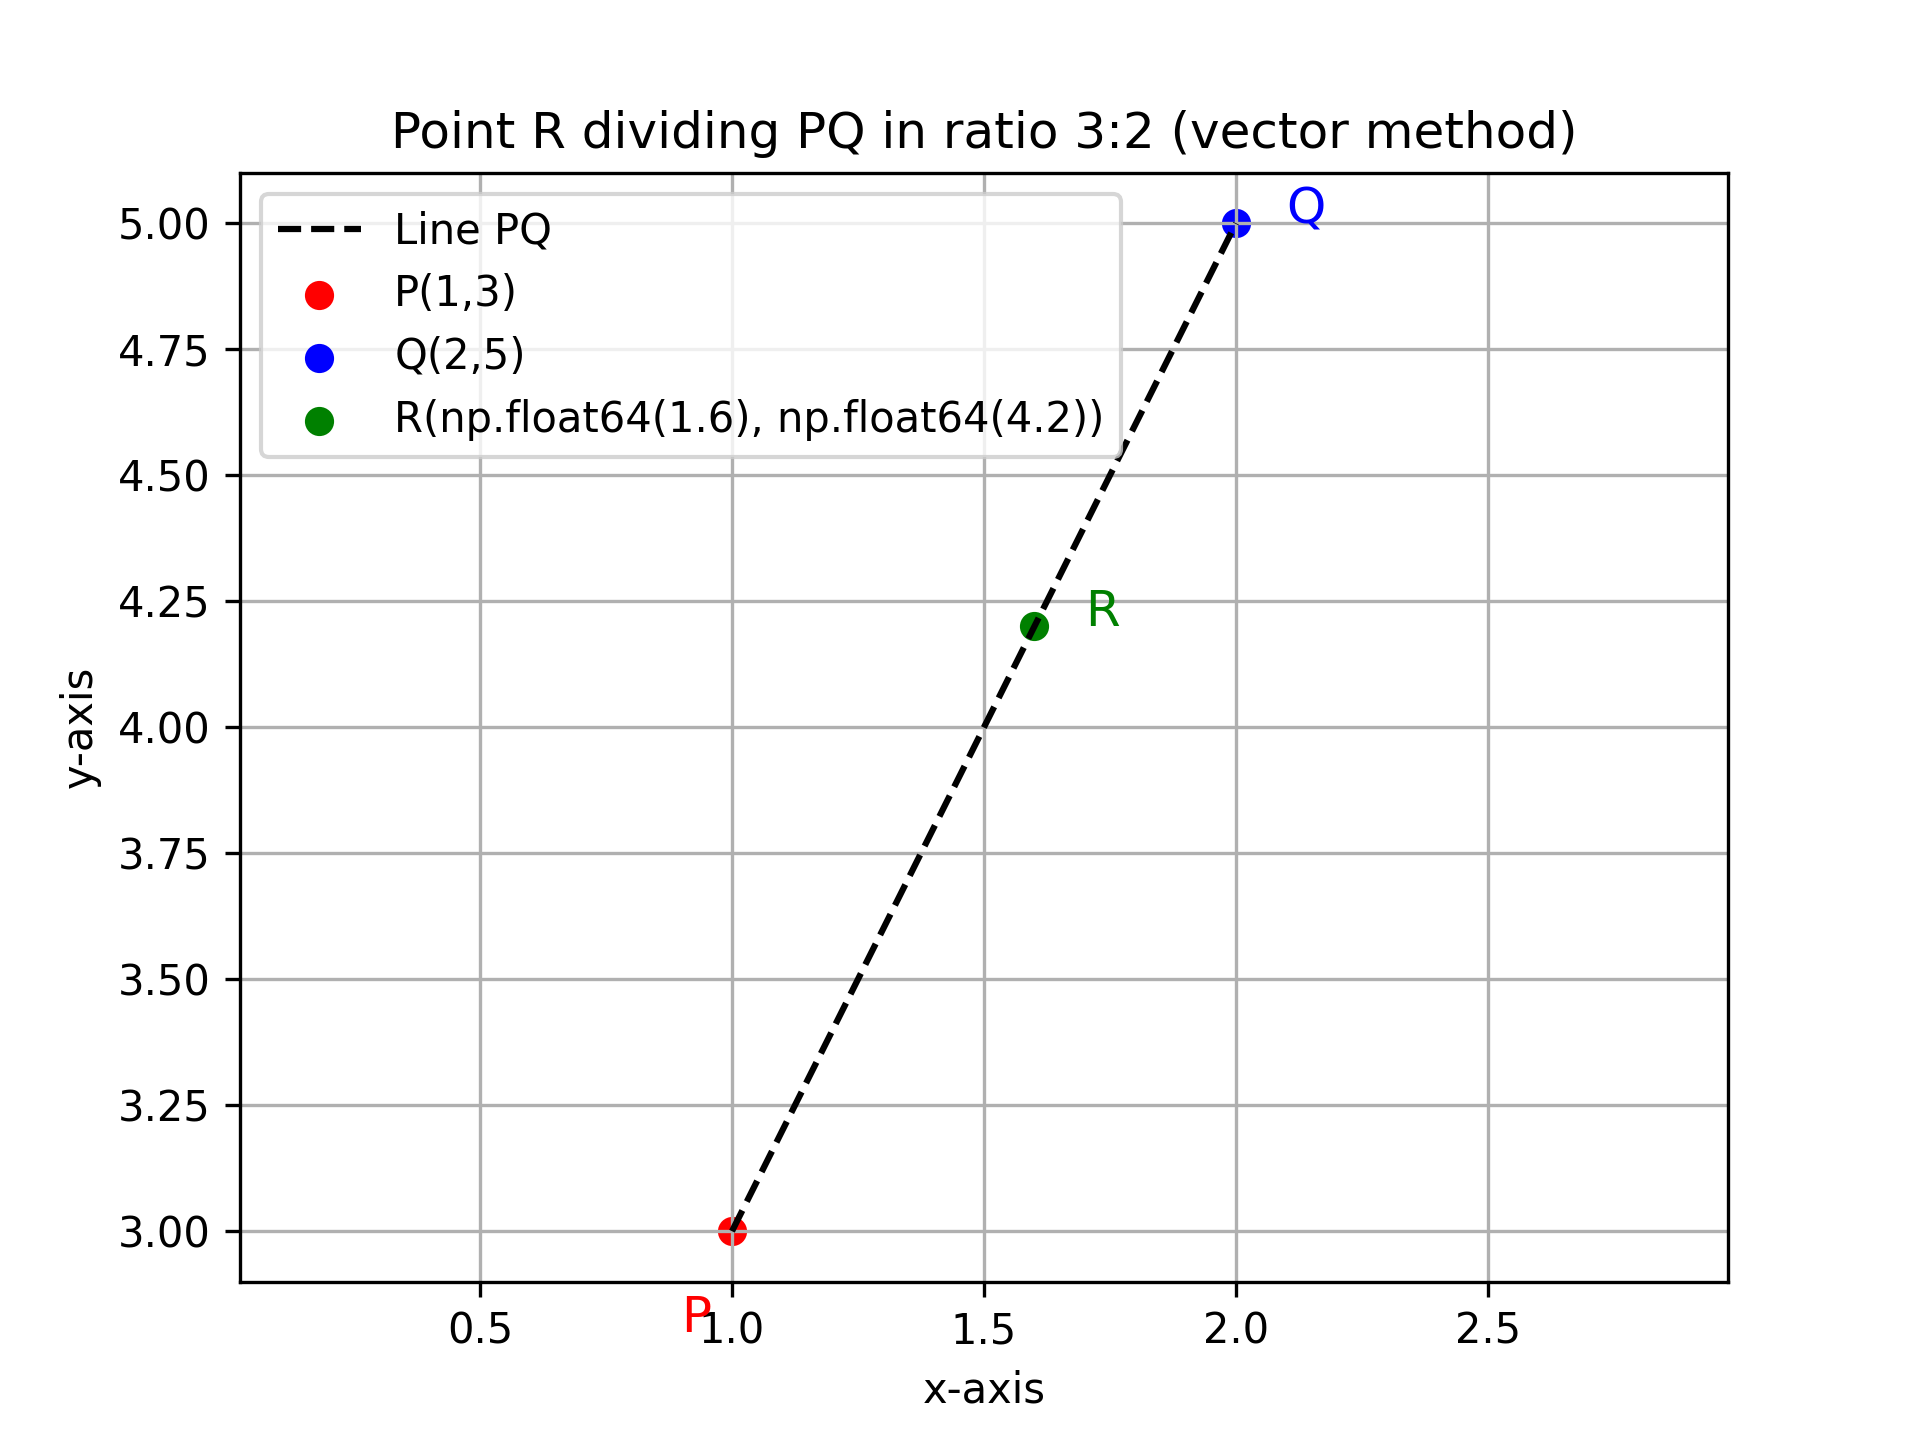
\includegraphics[width=0.9\columnwidth]{figs/PQ_R_plot.png}
   \end{figure}
\end{frame}

\begin{frame}[fragile]
    \frametitle{Code - C}
    The code to find the coordinates of point R is
    \begin{lstlisting}
#include <stdio.h>

void point_on_segment2d(const double P[2], const double Q[2], double lambda, double R[2]) {
    R[0] = P[0] + lambda * (Q[0] - P[0]);
    R[1] = P[1] + lambda * (Q[1] - P[1]);
}




\end{lstlisting}
\end{frame}

\begin{frame}[fragile]
    \frametitle{Code - Python(with shared C code)}
    The code to obtain the required plot is
    \begin{lstlisting}

import ctypes
import numpy as np
import matplotlib.pyplot as plt

# Load the shared library (Linux name shown here)
lib = ctypes.CDLL("./librpoint.so")

# Tell ctypes the C function signature
lib.point_on_segment2d.argtypes = [
    ctypes.POINTER(ctypes.c_double),  # P
    ctypes.POINTER(ctypes.c_double),  # Q
    ctypes.c_double,                  # lambda
    ctypes.POINTER(ctypes.c_double)   # R
]
lib.point_on_segment2d.restype = None

\end{lstlisting}
\end{frame}
\begin{frame}[fragile]
\frametitle{Code - Python(with shared C code)}
\begin{lstlisting}

# Data
P = np.array([1.0, 3.0], dtype=np.float64)
Q = np.array([2.0, 5.0], dtype=np.float64)
lam = 3.0/5.0
R = np.zeros(2, dtype=np.float64)

# Call C
lib.point_on_segment2d(
    P.ctypes.data_as(ctypes.POINTER(ctypes.c_double)),
    Q.ctypes.data_as(ctypes.POINTER(ctypes.c_double)),
    lam,
    R.ctypes.data_as(ctypes.POINTER(ctypes.c_double))
)

print("R from C:", tuple(R))  # Expect (1.6, 4.2)

\end{lstlisting}
\end{frame}
\begin{frame}[fragile]
\frametitle{Code - Python(with shared C code)}
\begin{lstlisting}

# Plot
plt.plot([P[0], Q[0]], [P[1], Q[1]], 'k--', label="PQ")
plt.scatter(*P, color='red', label="P")
plt.scatter(*Q, color='blue', label="Q")
plt.scatter(*R, color='green', label="R")
plt.legend()
plt.title("R=P+(3/5)(Q-P)")

# Save first, then show
plt.savefig("/sdcard/ee1030-2025/ai25btech11032/Matgeo/1.4.2/figs/PQ_R_plotnew.png", dpi=300)
plt.show()


\end{lstlisting}
\end{frame}
\begin{frame}[fragile]
\frametitle{Code - Python only}
\begin{lstlisting}
import numpy as np
import matplotlib.pyplot as plt

# Define vectors
P = np.array([1, 3])
Q = np.array([2, 5])


lam = 3/5
R = P + lam * (Q - P)

\end{lstlisting}
\end{frame}
\begin{frame}[fragile]
\frametitle{Code - Python only}
\begin{lstlisting}


# Plot PQ Line
plt.plot([P[0], Q[0]], [P[1], Q[1]], 'k--', label="Line PQ")

# Plot points
plt.scatter(*P, color='red', label="P(1,3)")
plt.scatter(*Q, color='blue', label="Q(2,5)")
plt.scatter(*R, color='green', label=f"R{tuple(R)}")

# Annotate points
plt.text(P[0]-0.1, P[1]-0.2, "P", fontsize=12, color='red')
plt.text(Q[0]+0.1, Q[1], "Q", fontsize=12, color='blue')
plt.text(R[0]+0.1, R[1], "R", fontsize=12, color='green')

\end{lstlisting}
\end{frame}
\begin{frame}[fragile]
\frametitle{Code - Python only}
\begin{lstlisting}

# Style
plt.xlabel("x-axis")
plt.ylabel("y-axis")
plt.title("Point R dividing PQ in ratio 3:2 (vector method)")
plt.legend()
plt.grid(True)
plt.axis("equal")

# Save plot to file
plt.savefig("PQ_R_plot.png", dpi=300)   # Saves in current folder
# plt.savefig("PQ_R_plot.pdf")         # Alternative format

plt.show()




    \end{lstlisting}
\end{frame}
\end{document}
